\chapter*{Introduction}
\addcontentsline{toc}{chapter}{Introduction}
%
\linenumbers
%
Modern society faces a wide range of challenges that require complex and multifaceted solutions. The challenges posed by climate change and the necessity for clean energy in order to reduce greenhouse gas emissions intersect with the goals of economic growth and the global exchange of information, goods and people. Unprecedented issues are emerging from this increasingly technologically advanced and interconnected civilization. 

This PhD work was initiated amidst the most impactful public health crisis of our time, the COVID-19 pandemic. Despite all the negative facets of this pandemic, it unexpectedly gave a boost to a specific market : the emerging technology of deep ultraviolet violet light-emitting diodes (UVC LEDs), and the market is predicted to grow five-fold.\cite{Yole} Indeed the deep UV light, \textit{i.e.} with wavelengths ranging from 100 to 280 nm, has been demonstrated to inactivate the coronavirus accountable for the disease, thus making it harmless.\cite{GERCHMAN2020112044} Besides surface disinfection, UVC LEDs have many applications in water and air depolution, agriculture, printing and more.\cite{hsu2021perspectives} The material studied in this thesis, hexagonal Boron Nitride, is a candidate of choice for the elaboration of UVC LEDs due to its bright light emission in the deep ultraviolet.

% above is to keep
% below is to correct
This is a recent example of how technological innovations emerging from scientific research in materials science could provide a means to overcome the challenges of modern society. The European Union is supporting such research notably with the Flagship projects, that are large scale research initiatives with an accent on transfer technologies to industry. Three out of the four Flagship projects are closely related to materials sciences : Batteries30+ for the development of efficient and compact energy storage, Quantum Technologies for the quantum computers and algorithms and Graphene, whose focus is on two-dimensional materials. All of these, along with the ITER project for nuclear fusion, are research projects that could provide a means to produce clean energy. In all of these scientific fields, theory and numerical simulations are essential to support the experimental discovery of materials and the technological production of new products. This is especially relevant in Condensed Matter Physics which is the object of this thesis. Since the discovery of Graphene and its exceptional properties by Novoselov and Geim,\cite{graphene} the two-dimensional (2D) materials such as Graphene, black Phosphorus, transition metal dicalchogenides (TMDs) and hexagonal Boron Nitride (hBN) attracted a lot of attention. Indeed these exhibit a range of electronic and optical properties which allows to design devices for different applications, especially when stacking different layers together and forming the so-called van der Waals heterostructures.\cite{something} The obtained components are then very compact and fit very well in the technological trend of device miniaturization.

With the variety of optical and electronic properties offered by all the existing monolayers, and the possibility to engineer them with factors such as stacking of different layers,\cite{sponza2018direct} twisting angle them,\cite{latil2023structural, impellizzeri2022electronic} and straining\cite{blundo2021strain} as well as their interaction with substrates, the possibilities for devices are almost limitless. In this ecosystem, hexagonal Boron Nitride is a candidate of choice for its structural, electronic and optical properties.

% 
\subsection{Paragraph on the properties of hBN}
Generalities about hBN \\
AA'-hBN is stable at room temperature and ambient pressure
hBN : hig gap, pDOS of valence at K is mostly Nitrogen, $\pi$ orbital(overlap of $p_z$, bonding)  . pDOS of conduction at M is mostly Boron, $\pi^*$ orbital (overlap of $p_z$ with opposite coefficient, antibonding)\\
%We could compute phonon-assisted absorption but the phonon satellites are very small wrt to the main peaks so when they overlap, they are not visible.\\


\subsection{Explain luminescence}
Optical measurements are an efficient way to characterize materials and reveal the microscopic, quantum, interplay between electronic wavefunctions and electromagnetic field of light, and collective quantum effects in the crystal.\cite{something} In particular, spontaneous emission of light after an excitation, known as \textit{luminescence}, is the key property for the elaboration of light-emitting diodes. 

For spontaneous light emission to happen in a semiconductor or insulator, there needs to be excited electrons populating the conduction band. The excitation can have different forms. It can be done with the electromagnetic field of external light, then the process is called photoluminescence. If the electrons are excited by an external beam of electrons colliding with the crystal, it is called cathodoluminescence. If they are excited by an external electric field, it is called electroluminescence, \textit{et caetera}. When the electrons are promoted to the higher-energy conduction bands, they leave an empty state in the valence band. This empty state can be thought of as a \textit{hole} in the Fermi sea of the valence states. It propagates with the opposite of the electron's momentum and has a negative effective mass. For light to be emitted, the excited electrons need to de-excite and go back to the empty states. We speak of radiative recombination of an electron-hole pair. When the hole and the electron have the same momentum (and the same spin and symmetry) the radiative recombination can happen because the emitted light carries an almost zero momentum, hence respecting momentum conservation. The energy difference between the electron and the hole corresponds to the frequency of emitted light, multiplied by $\hbar$. 
However when the bottom of the conduction band is not at the same momentum than the top of the valence band, the light emission cannot happen directly because of momentum conservation. There needs to be a second-order process to exchange momentum. The excited electron can transfer its momentum to another one and then recombine with the hole. This process is known as Auger-Meitner recombination.\cite{somethingKioupakis} Otherwise, the momentum exchange can be done by absorbing or emitting a phonon, hence gaining or losing energy and momentum and finally recombine radiatively. This is known as a phonon-assisted transition and it is the process that is studied in this thesis. 

Luminescence is often thought of as the reverse process of light absorption. Indeed in absorption, light with a frequency higher than the gap can excite electrons and promote them to the conduction band, with almost zero transfer of momentum. In the case of phonon-assisted transitions, the electron can be promoted to the conduction band at another momentum, thanks to the absorption or emission of a phonon. 

Because of this similarity, the spectra of absorption and of luminescence are quasi symmetrical for direct transitions. The asymmetry come from the phonon broadening of the electron density of states, known as the Stokes shift. However for phonon-assisted transitions, the spectra can look very different, as illustrated by the experimental results presented in Fig. \textcolor{red}{Figure}. For bulk hexagonal Boron Nitride, the states dominating the absorption is different from the one dominating the luminescence, which is at lower energy. Moreover, since the phonon-assisted transitions appear as multiple peaks, there is a strong asymmetry in the spectra. This will be explained in details in the body of this thesis.

Absorption is easy to obtain from calculation, but luminescence is harder since it is an out-of-equilibrium process. For hBN it is the opposite on the experimental side of things : since the gap is very large, one needs high-frequency lasers for absorption, or synchrotron radiation as in Fig. \textcolor{red}{fig abs hBN}. For luminescence it less dependent on the excitation so its easier, but still we need low temperature to be able to resolve all the phonon peaks individually. When talking about a single layer it is even harder since the intensity of emitted light is low. This explain the very recent apparition of luminescence spectra of monolayer hBN in scientific litterature.

In this thesis, we study the properties of different forms of hBN and develop theoretical and numerical methods with the aim of reproducing and predicting their luminescence spectra from \textit{ab initio} calculations.

\subsection{Scope of the thesis}
%
Chapter 1 introduces the theoretical framework in which our calculations are contained. It starts from the adiabatic approximation that states that the electronic and the atomic motions can be decoupled thanks to the mass difference between nuclei and electrons.

We then include a brief description of the widely used \acrfull{DFT}. In this theory the electrons are treated as independent particles evolving in a mean-field. It allows to compute the ground state density of the crystal and to obtain the equilibrium geometries, with a certain set of approximations. From there we extract the Kohn-Sham eigenvalues and wavefunctions. These eigenvalues give an approximation to the band structure and are the starting point of the more involved \acrfull{MBPT}. 

\acrshort{MBPT} is based on Green's functions and treats the many-body interactions as a perturbation of the independent-particle system. The main equations of this theory are the Hedin's equations, whose derivation is sketched in this first Chapter. Truncating this set of self-consistent equations by neglecting the electron-hole interaction gives on one hand the \acrfull{RPA} to account for the dynamical screening and on the other hand the \acrfull{GWA}. In the latter, the matrix product of the electronic propagator $G$ and the dynamically screened interaction $W$ gives the \textit{self-energy} $\Sigma$. It can be interpreted as a non-local, frequency-dependent potential that dresses the independent electrons with the interactions with other electrons, which is an improvement with respect to \acrshort{DFT}. They become \textit{quasiparticles}, whose evolution in time and space is easier to describe than the full many-electrons system.
With this we are able to obtain a more accurate band structure and simulate experiments that involve charged excitations -- \textit{i.e.} addition or removal of an electron of the system. 

However the neutral excitations of the many-electron system -- \textit{i.e.} an electron being excited but staying in the system -- are not well described at this point. To this end, the electron-hole interaction is reintroduced by computing the two-particle Green's function. This is the solution of the so-called \acrfull{BSE}. Starting from the $GW$ approximation, the \acrshort{BSE} can be formulated in the basis of \textit{excitons}, which are quasiparticles made of an electron-hole pair, bound together by the Coulomb interaction. From the \acrshort{BSE} one can obtain the response function of the system including excitonic effects, with the assumption that excitations are instantaneous in time and response to these excitations. This is known as the \textit{static} approximation. Excitons have been shown to play a significant role in the optical spectra of \acrshort{hBN} and indeed the \acrshort{BSE} description is in much better agreement with experiments compared to independent-particles or quasiparticles levels of theory, as can be seen in Fig. \textcolor{red}{Figure of absorption}. The link between microscopic excitonic quantities and macroscopic observables is presented in the middle of the first Chapter. 

Finally Chapter ends on the presentation of a perturbative method based on \acrshort{DFT} to obtain the vibrational properties of the crystal in the harmonic approximation, meaning that each atom is represented as an harmonic oscillator vibrating around its equilibrium position. It is called \acrfull{DFPT}. In second quantization, it gives a description of the vibration modes of the lattice in terms of quanta of vibration called \textit{phonons}. They are another type of quasiparticle, that is a collective excitation, with a definite frequency and wave vector, analogous to the crystal momentum of electrons. We can now reintroduce the coupling between nuclear and electronic motions and formulate the electron-phonon coupling in second quantization. We obtain the coupling matrix elements that are the probability amplitudes that a electron is scattered by a phonon from a given momentum-energy state into another, where the energy and momentum is exchanged with the phonon.  
\begin{figure}[h!b]
	\vspace{0.2cm}
	\setcapindent{2em}
	\centering
	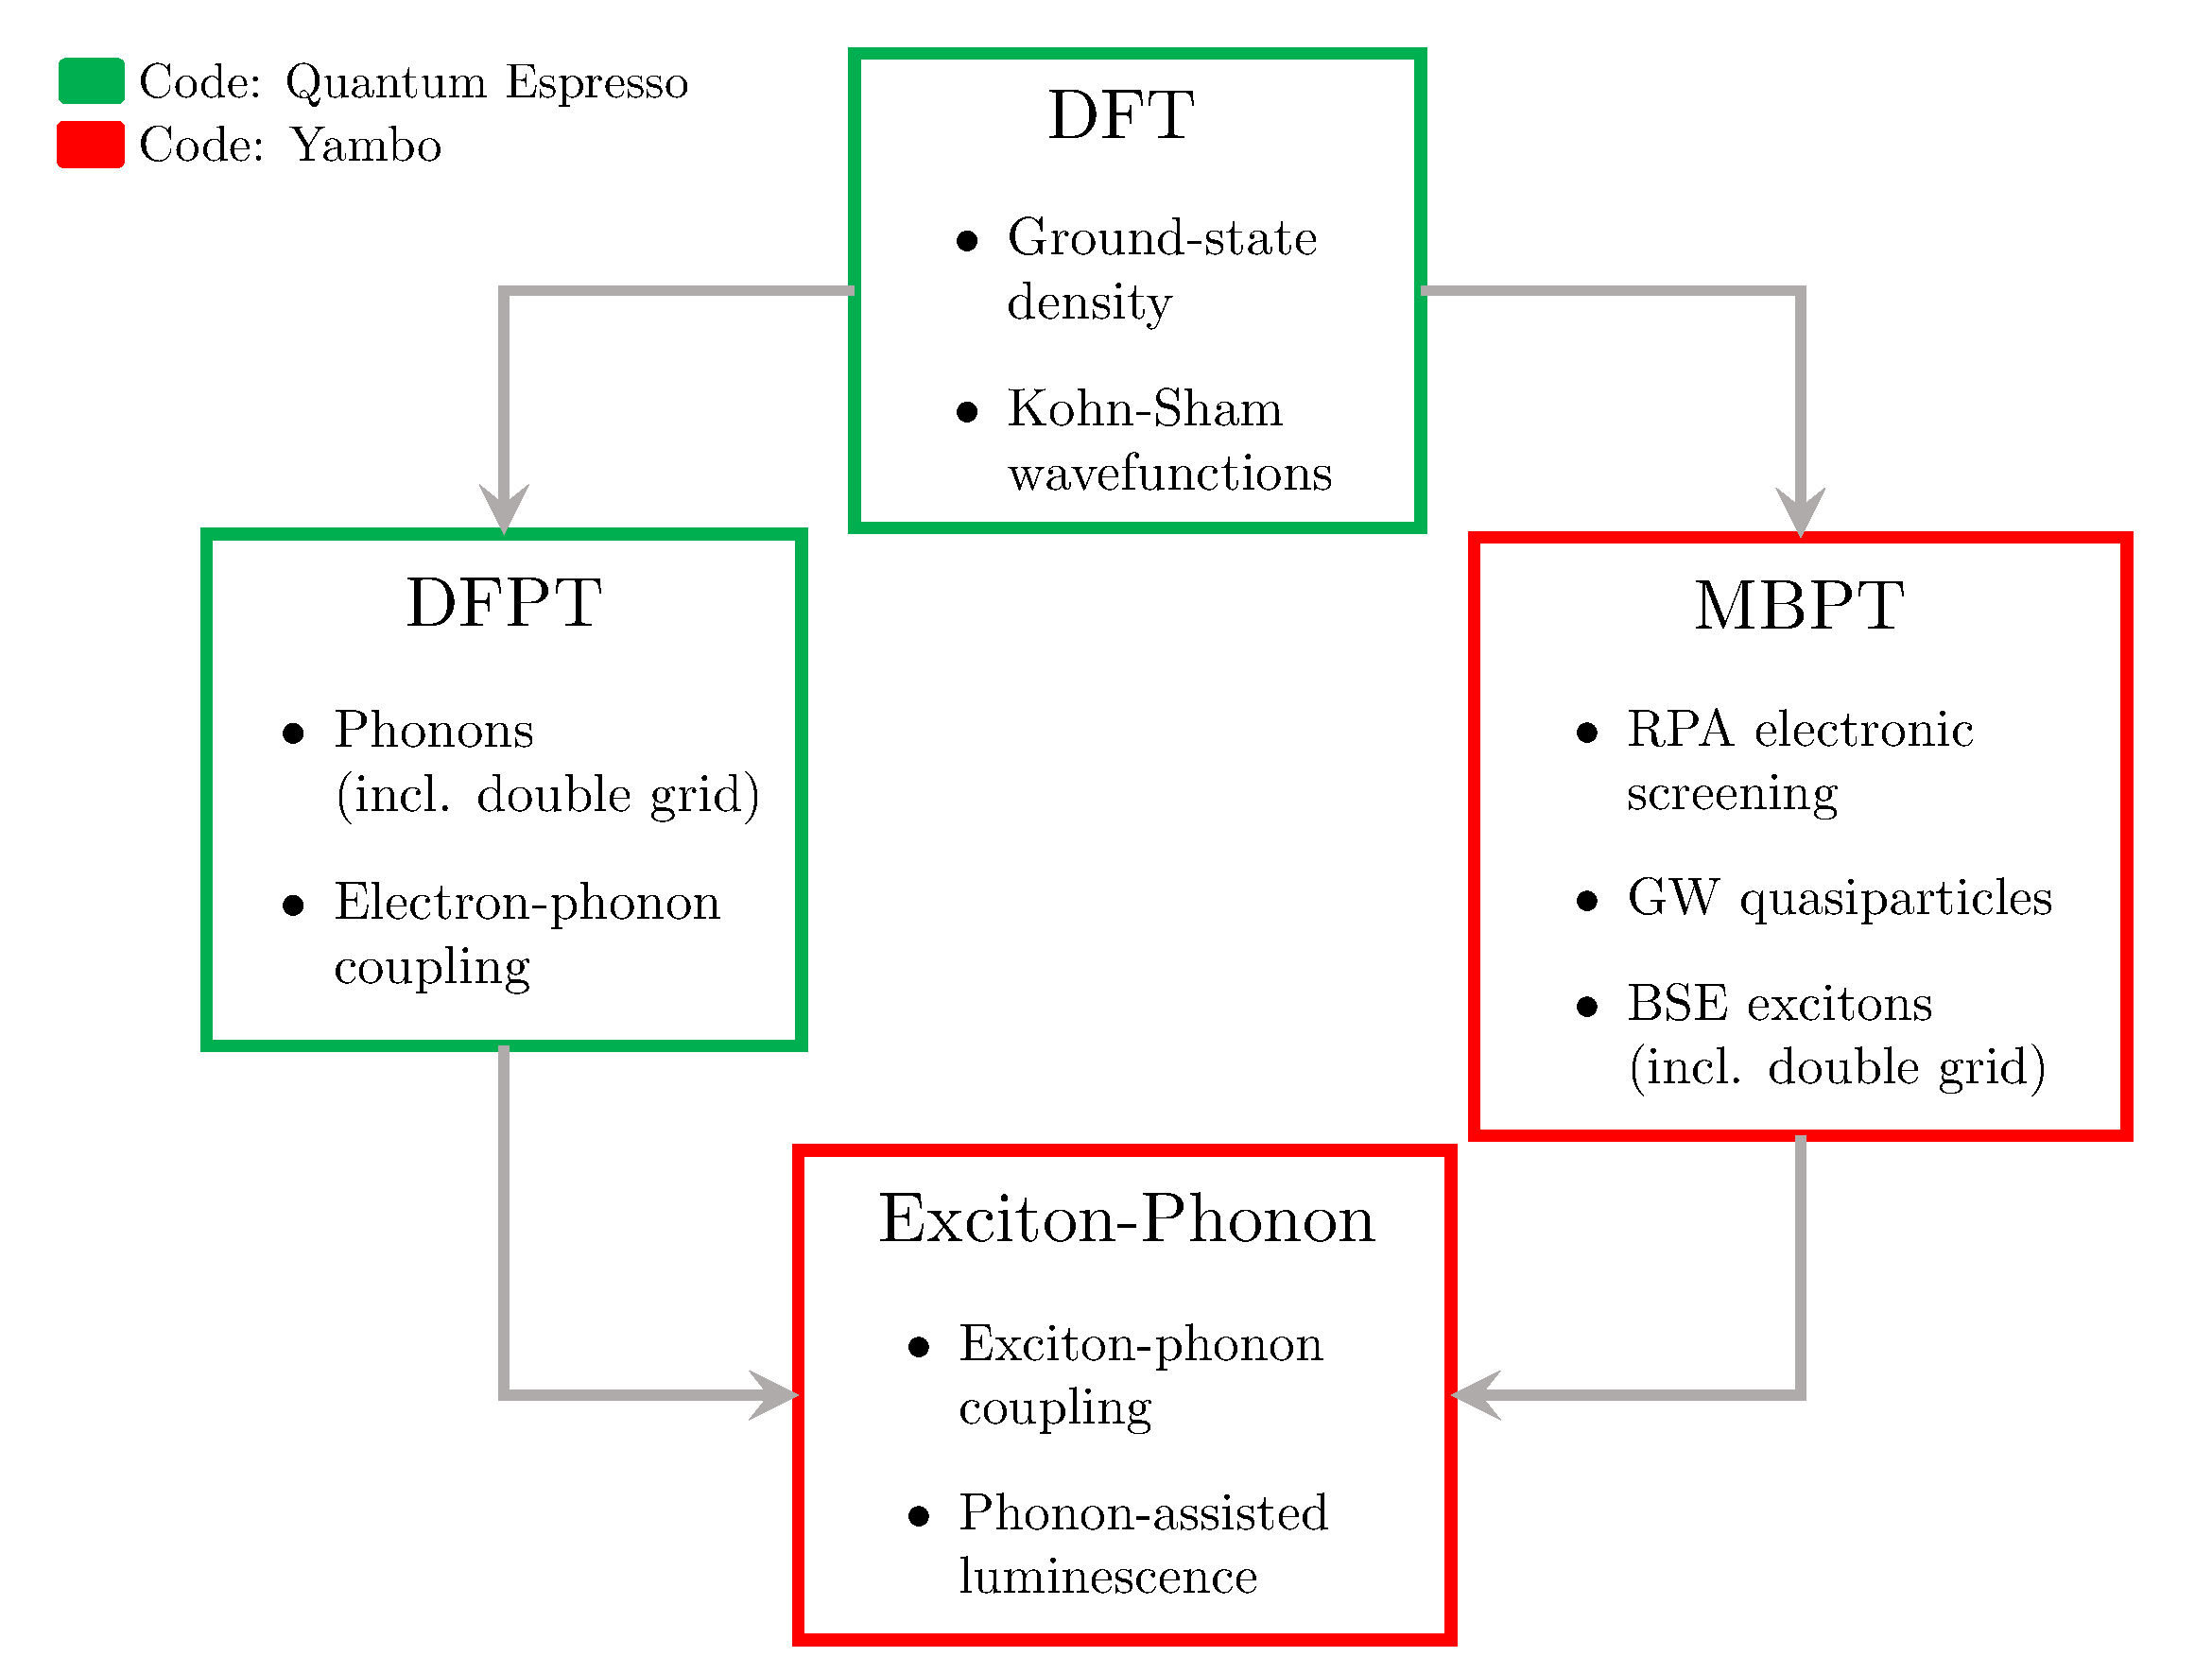
\includegraphics[width=0.9\textwidth]{workflow_detailed.pdf}
	\caption{Workflow of the calculations to compute exciton-phonon coupling and phonon-assisted luminescence. The green/red boxes indicate that we used \textsc{Quantum ESPRESSO} / \yambo~as simulation codes.}
	\label{fig:workflow}
\end{figure}

at the end of the description of chapter , put the workflow
after the workflow, talk about the way we compute excph coupling in the two Chapters

In condensed matter, the problem of exciton-phonon coupling and phonon-assisted luminescence is an old topic. The first studies date back to the 60s by Toyozawa \emph{et al.}\cite{toyozawa2003optical,toyozawa1964interband} and the first dynamical solution of the Bethe-Salpeter equation (BSE), the so-called Shindo solution, was proposed precisely to study the exciton-phonon problem.\cite{shindo1970effective}
More recently, this problem has been studied in different materials, from nanotubes\cite{perebeinos} to 2D crystals, and new methodologies were introduced, such as the cumulant Ansatz\cite{cudazzo2020first}, polaron transformation,\cite{feldtmann2009phonon} density matrix,\cite{brem2020phonon} two-particles Green's functions\cite{antonius2017theory} and real-time approach,\cite{paleari2022coupling} with the aim of deriving a modern formulation of exciton-phonon interaction and its related observables, such as phonon-assisted luminescence, within many-body perturbation theory (MBPT).

Theory of phonon-assisted optics : it exists. For instance, Williams-Lax theory that treats lattice-dependent band features and phonon-assisted transitions 
There is also Hallen-Bardeen-Blatt and Heine-Cardona but I don't know too much about them.
Besides, some models of exciton-phonon coupling exists also, some specifically for luminescence, but they are computationally expensive for real materials.
Zacharias and Giustino (+ Jordan?) derive a formalism based on Williams-Lax to describe phonon-assisted absorption 

==> there is a need for exciton-phonon coupling and phonon-assisted optics from first principles. In Chapters 2 and 3, two different approaches are presented in Sections \ref{sec:excph_fdd} and \ref{sec:excph_ai}. The first one consists in calculating the response function correction due to exciton-phonon coupling from finite differences, by displacing atoms in supercells. The second one is a more general approach based on \acrshort{MBPT}, in which a dynamical correction induced by electron-phonon coupling is added as a perturbation to the static Bethe-Salpeter kernel. Thanks to this \textit{ab initio} framework, the scattering of every exciton with every phonon mode can be computed, over the whole Brillouin Zone. These calculations are done in the unit cell.
Both approaches allow to compute the exciton-phonon coupling. Then, the absorption can be obtained after post-processing of a standard \acrshort{BSE} calculation. To obtain the luminescence spectra, we use the van Roosbroeck -- Shockley relation for both cases.
Exciton-phonon in hBN are not only possible, but likely due to strong electron-phonon coupling. Verified experimentally by the External Quantum Efficiency comparable to direct gap materials.\\


\subsection{Structure}
describe chapter 2
describe chapter 3
appendices


% ETSF webinar of Fulvio
% indirect bandgap only; we can write the response function with derivatives of the response function because we consider only phonon-assisted transitions; need supercells
% PLE (propto absorption) or absorption and PL are not symmetric, as expected for direct gaps
% the minimum exciton at T is the degenerate dark state at Gamma which splits
% for absorption, the bright exciton overlaps with the phonon replicas and it is so bright that we don't see them 

% UV to kill coronavirus : https://doi.org/10.1016/j.jphotobiol.2020.112044
%Hsu, Tsung-Chi, et al. "Perspectives on UVC LED: Its progress and application." Photonics. Vol. 8. No. 6. MDPI, 2021.
% In 2019, the total market for UV LEDs reached US\$ 144M,mostly driven by water disinfection. Following the COVID-19 outbreak, demand for UVGI greatly increased, and a five-fold growth in surface disinfection applications has been predicted by Yole Développement, leading to a total UV LED market of up to US\$ 300M 
% cite : Yole-Developpement 2020UVC LEDs : One Solution toContain the COVID-19 Pandemic(available at:http://www.yole.fr/iso_upload/News/2020/PR_UV_LED_MarketUpdate_YOLEGROUP_Oct2020.pdf)
